\section{Development Workflow}

% input: protocol, role, target
% then: verify well-formedness
% then: obtain EFSM for role
% then: parse EFSM
% then: generate code for said target
% output: API

We motivate our development workflow from previous work 
\cite{PureScript2019} by extending the \fancyname{Scribble} toolchain
and generating APIs that integrate developer implementation
into the EFSM execution.

We visualise the workflow in \cref{fig:devworkflow} 
and provide a brief overview:

\begin{enumerate}

\item The developer supplies the communication protocol written in
\fancyname{Scribble} (\cref{subsection:scribble}), 
stating the role (hereafter \textit{endpoint})
to generate APIs for,
and the code generation \textit{target} 
(i.e. whether the role runs on the server or the web browser).

\item \fancyname{SessionTS} delegates to the 
\fancyname{Scribble} toolchain for verifying the well-formedness of
the protocol and expects to receive a DOT graph representation of
the endpoint FSM (\cref{subsection:efsm}). 
\fancyname{SessionTS} parses the endpoint's 
interactions from the DOT graph and generates TypeScript APIs
for the developer (\cref{subsection:apigen}) 
tailored to the specified target.

\item The developer implements their web application using the
generated APIs. Implementations that pass the type-checking phase
of the TypeScript Compiler are guaranteed to be free from 
communication errors by session type theory.

\end{enumerate}

\begin{figure}[!ht]
\centering
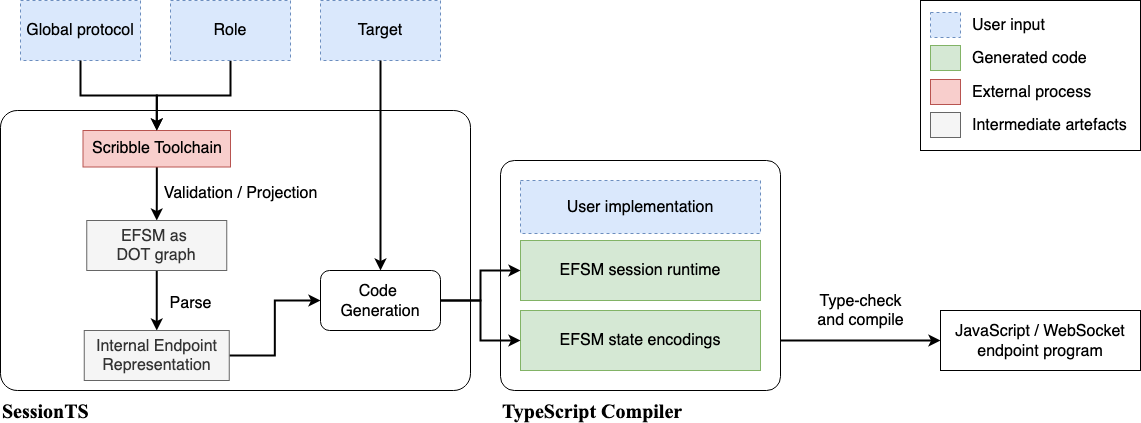
\includegraphics[width=\textwidth]{DevelopmentWorkflow}
\captionof{figure}{Overview of \fancyname{SessionTS} Development Workflow}
\label{fig:devworkflow}
\end{figure}

\subsection{Protocol Specification with \fancyname{Scribble}}
\label{subsection:scribble}

\begin{itemize}
\item see notes from PLACES paper on scribble
\item scribble language definition (unless already in background)
\end{itemize}

\subsection{From \fancyname{Scribble} to EFSM}
\label{subsection:efsm}

\begin{itemize}
\item scribble validates the protocol
\item use flag to obtain EFSM representation
\item DOT graph output
\item parse in python -- use open-source library for this
\end{itemize}

\subsection{Code Generation}
\label{subsection:apigen}

\begin{itemize}
\item api generation is a function of the EFSM representation
\item traditional methods -- visitor pattern on the EFSM and using stringbuilder to build the file
\item templating library is more suitable to decouple the ``presentation'' (how the code should look) from the ``content'' (the EFSM which is used to build the code)
\item strategy pattern to support the two required build targets (in node and react)
\end{itemize}